\chapter{Zusammenfassung und Ausblick}
In dieser Arbeit sollte ein System entwickelt werden, das eine Schnittstelle zwischen der Anwendung und der Roboterkontrollarchitektur implementiert (siehe \autoref{fig:gui_puzzel}). 

 \begin{figure}[H]
 \centering
 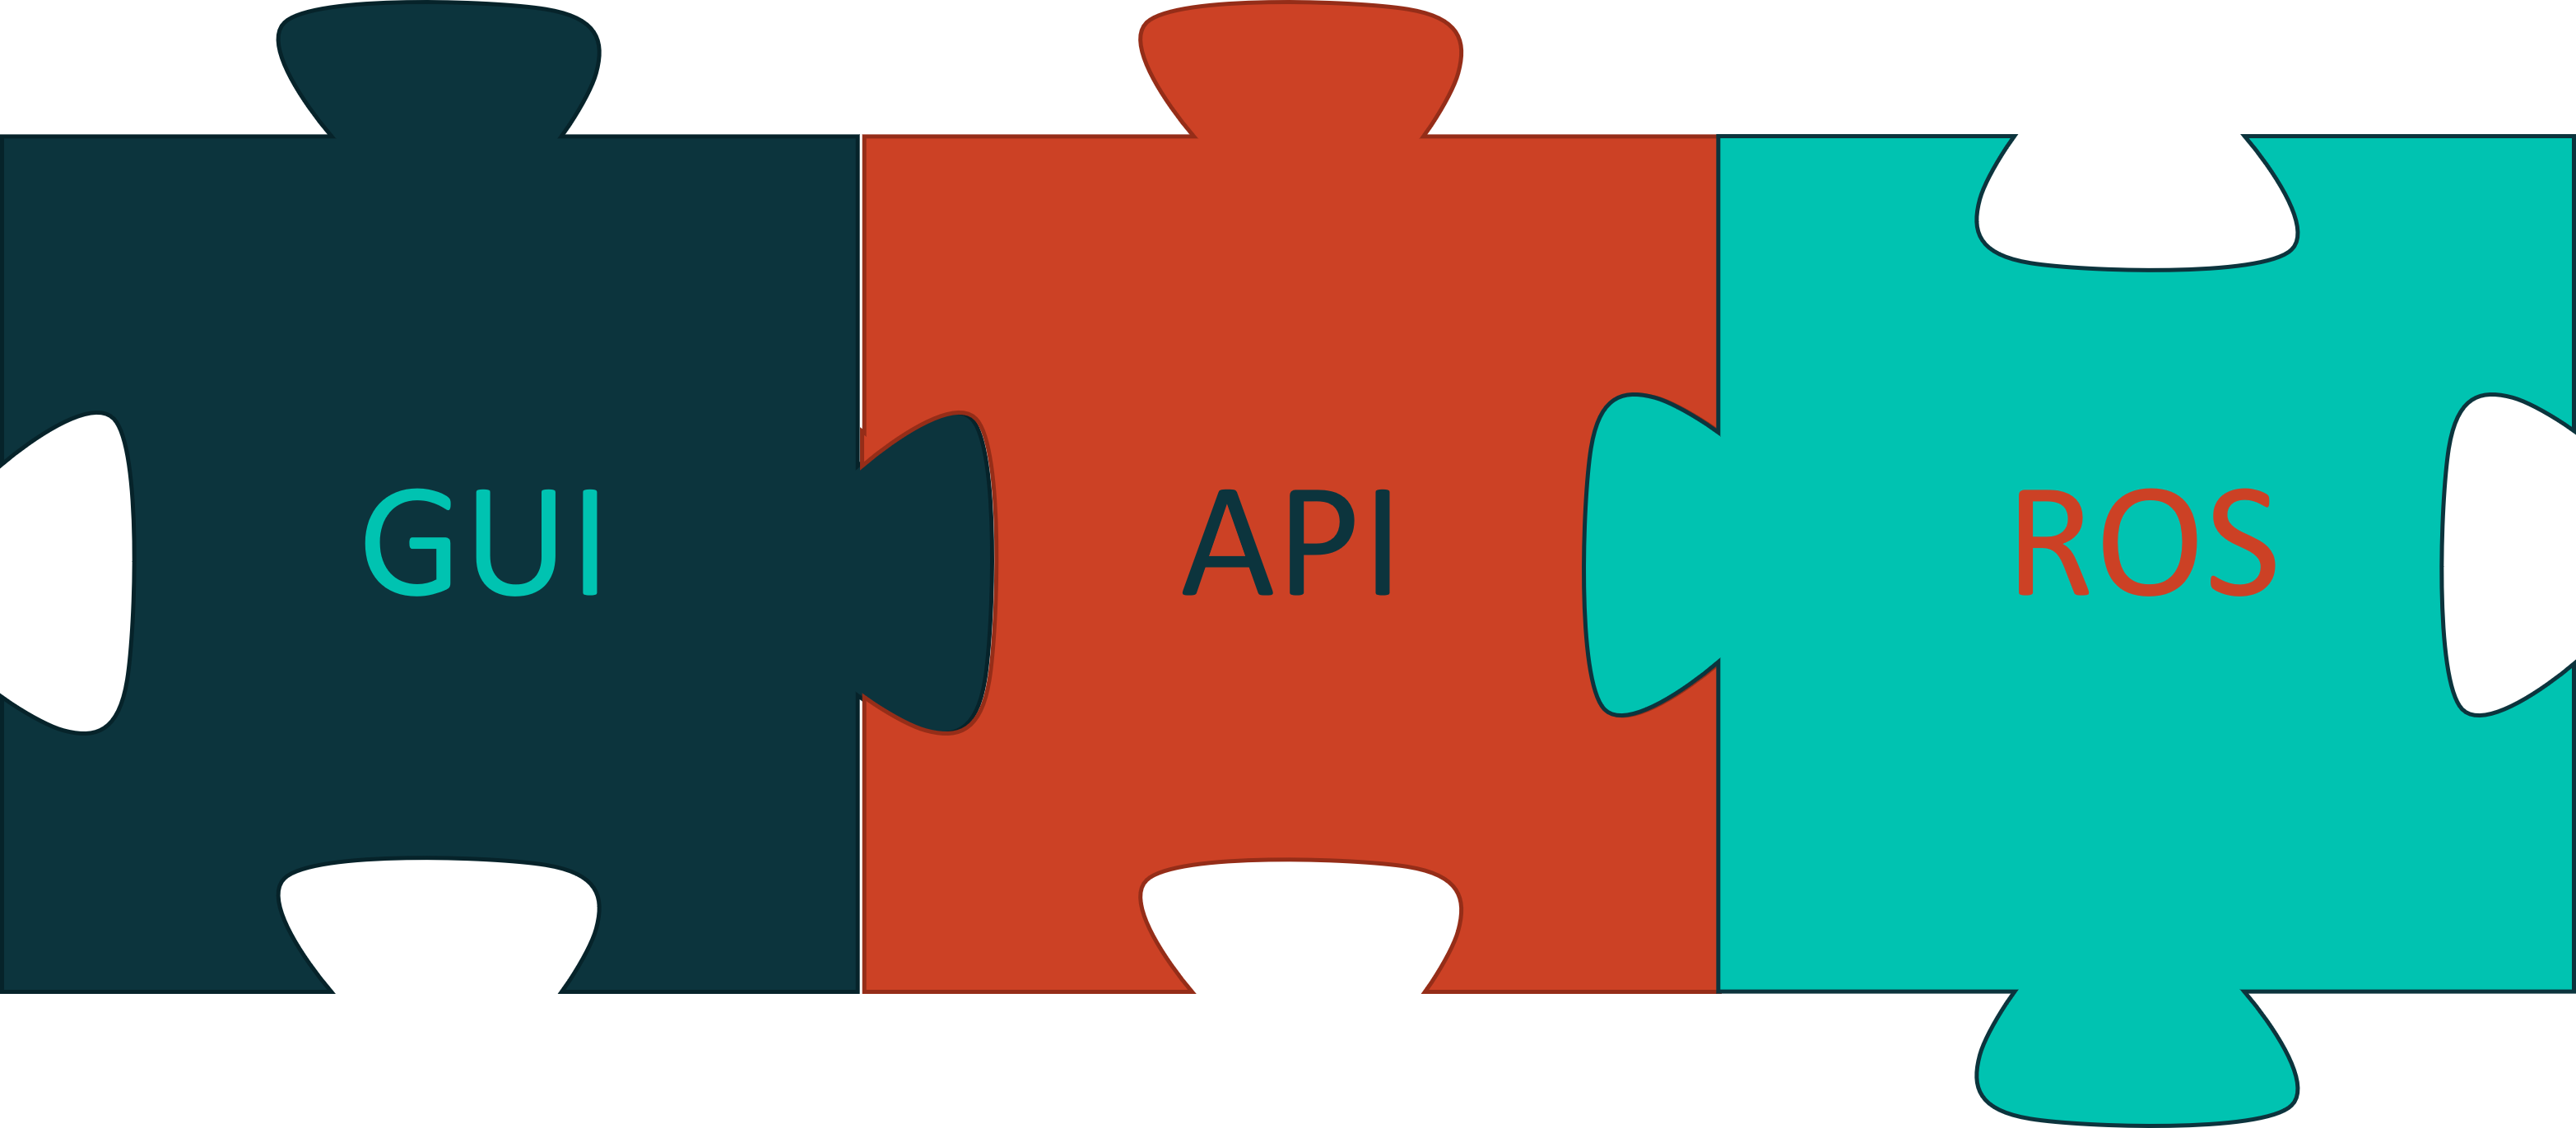
\includegraphics[width=\linewidth]{Bilder/Ausblick/api_bridge.png}
 \caption{Darstellung der Schnittstelle}
 \label{fig:gui_puzzel}
\end{figure}

Dabei sollte das System als ein Exponat vermarktet werden. Der Markt dafür sind Bildungseinrichtungen. So soll spielerisch die Intelligenz von mobilen Robotern vermittelt werden. Ein weiterer Einsatzbereich ist die Vermittlung von Informationstechnologie. So kann die Benutzeroberfläche als Lehrmaterial gestaltet werden, um Schüler und Studierenden das Programmieren oder das technische Denken spielerisch zu transportieren. Dies würde somit die alteingesessenen Methoden mit Büchern oder Simulationen ergänzen. Das System in dieser Arbeit verwendet verschiedene Sensoren, die im Laufe des Projektes immer wieder ergänzt wurden, um mehrere Möglichkeiten abzudecken. So konnte mithilfe eines rotierenden Laserscanners der Abstand zu Hindernissen gemessen werden und im Programm die Hindernisse vermieden werden. Dies ermöglichte auch eine relative Navigation des mobilen Roboters. Des Weiteren wurden Ultraschallsensoren seitlich des Roboters integriert, um dem Pledge- Algorithmus ausreichende Daten zu liefern. Dazu wurde eine separate Implementierung vorgenommen, um den Sensor abzufragen und über ROS die Werte zu veröffentlichen. Die Fähigkeiten von mobilen Robotern sollten mithilfe des Befreiungsalgorithmus im Labyrinth aufgezeigt werden. Dazu wurde der Plegde- Algorithmus verwendet, der auch schon bewiesen hatte, dass er immer einen Ausweg findet, wenn ein Ausweg aus dem Labyrinth existiert. Das Ganze wurde nur prototypisch als Zustandsautomat entwickelt und nur einzelne Teile wurden getestet. Im kompletten zusammenhängenden Ausmaß wurden dazu keine Tests durchgeführt. Die Arbeit entstand in der Zusammenarbeit mit der Firma Kurt Hüttinger GmbH und somit sollte das System als ein komplettes Exponat vermarktet werden. So war bei der Entwicklung klar, dass es keinen wirklichen Ausweg aus dem Labyrinth geben wird. Um trotzdem ein Ziel zu definieren, wurde das System mit einer Kamera erweitert, damit durch QR-Codes das Ziel markiert werden kann. Diesbezüglich wurde ein separates Modul entwickelt, das mithilfe von ZBar, QR-Codes aus Livebilddaten ausliest und über ROS veröffentlicht. Dadurch kann das Ende für den Algorithmus detektiert werden. Das Bindeglied der ganzen einzelnen Teile ist das API. Das API verbindet die ganzen Module miteinander und ermöglich durch Standard-Netzwerkprotokolle die Bedienung des mobilen Roboters.\\
Das ganze System wurde an die Firma Kurt Hüttinger GmbH \& Co. KG übergeben. Die Schnittstelle kann so eingesetzt werden. Die Firma kann das System mit weiteren Funktionalitäten erweitern, da es bausteinförmig und objektorientiert aufgebaut ist.\\
Dadurch das die Implementierung relativ modular und objektorientiert aufgebaut ist, können leicht weitere Intelligenzen eingebaut werden. So kann als Ausblick genannt werden die Kartierung vom Labyrinth mit SLAM und im Anschluss der Kartierung kann die Navigation mithilfe von weiteren Algorithmen für Pfadfindung erfolgen. Dazu kann der A-Star oder Dijkstra Algorithmus genannt werden, die als Suchalgorithmus dienen. Da auch künstliche Intelligenz immer mehr gefragt und eingesetzt wird, kann dieses System auch mit einer künstlichen Intelligenz erweitert werden, wie zum Beispiel mit einer Kamera, die Objekte und Gegenstände erkennt und je nachdem Entscheidungen trifft. So können auch Rampen eingebaut werden und der mobile Roboter erkennt diese, fährt über die Rampe, wird also diese nicht mehr als Hindernis betrachten. Im Allgemeinen kann das Projekte noch mit vielen Möglichkeiten und Intelligenzen erweitert werden. 